% This template has been tested with LLNCS DOCUMENT CLASS -- version 2.20 (10-Mar-2018)

% !TeX spellcheck = en-US
% !TeX encoding = utf8
% !TeX program = pdflatex
% !BIB program = bibtex
% -*- coding:utf-8 mod:LaTeX -*-

% "a4paper" enables:
%  - easy print out on DIN A4 paper size
%
% One can configure a4 vs. letter in the LaTeX installation. So it is configuration dependend, what the paper size will be.
% This option  present, because the current word template offered by Springer is DIN A4.
% We accept that DIN A4 cause WTFs at persons not used to A4 in USA.

% "runningheads" enables:
%  - page number on page 2 onwards
%  - title/authors on even/odd pages
% This is good for other readers to enable proper archiving among other papers and pointing to
% content. Even if the title page states the title, when printed and stored in a folder, when
% blindly opening the folder, one could hit not the title page, but an arbitrary page. Therefore,
% it is good to have title printed on the pages, too.
%
% It is enabled by default as the springer template as of 2018/03/10 uses this as default

% German documents: pass ngerman as class option
% \documentclass[ngerman,runningheads,a4paper]{llncs}[2018/03/10]
% English documents: pass english as class option
\documentclass[english,runningheads,a4paper]{llncs}[2018/03/10]

%% If you need packages for other papers,
%% START COPYING HERE

% Set English as language and allow to write hyphenated"=words
%
% In case you write German, switch the parameters, so that the command becomes
%\usepackage[english,main=ngerman]{babel}
%
% Even though `american`, `english` and `USenglish` are synonyms for babel package (according to https://tex.stackexchange.com/questions/12775/babel-english-american-usenglish), the llncs document class is prepared to avoid the overriding of certain names (such as "Abstract." -> "Abstract" or "Fig." -> "Figure") when using `english`, but not when using the other 2.
% english has to go last to set it as default language
\usepackage[ngerman,main=english]{babel}
%
% Hint by http://tex.stackexchange.com/a/321066/9075 -> enable "= as dashes
\addto\extrasenglish{\languageshorthands{ngerman}\useshorthands{"}}
%
% Fix by https://tex.stackexchange.com/a/441701/9075
\usepackage{regexpatch}
\makeatletter
\edef\switcht@albion{%
  \relax\unexpanded\expandafter{\switcht@albion}%
}
\xpatchcmd*{\switcht@albion}{ \def}{\def}{}{}
\xpatchcmd{\switcht@albion}{\relax}{}{}{}
\edef\switcht@deutsch{%
  \relax\unexpanded\expandafter{\switcht@deutsch}%
}
\xpatchcmd*{\switcht@deutsch}{ \def}{\def}{}{}
\xpatchcmd{\switcht@deutsch}{\relax}{}{}{}
\edef\switcht@francais{%
  \relax\unexpanded\expandafter{\switcht@francais}%
}
\xpatchcmd*{\switcht@francais}{ \def}{\def}{}{}
\xpatchcmd{\switcht@francais}{\relax}{}{}{}
\makeatother

\usepackage{ifluatex}
\ifluatex
  \usepackage{fontspec}
  \usepackage[english]{selnolig}
\fi

\iftrue % use default-font
  \ifluatex
    % use the better (sharper, ...) Latin Modern variant of Computer Modern
    \setmainfont{Latin Modern Roman}
    \setsansfont{Latin Modern Sans}
    \setmonofont{Latin Modern Mono} % "variable=false"
    %\setmonofont{Latin Modern Mono Prop} % "variable=true"
  \else
    % better font, similar to the default springer font
    % cfr-lm is preferred over lmodern. Reasoning at http://tex.stackexchange.com/a/247543/9075
    \usepackage[%
      rm={oldstyle=false,proportional=true},%
      sf={oldstyle=false,proportional=true},%
      tt={oldstyle=false,proportional=true,variable=false},%
      qt=false%
    ]{cfr-lm}
  \fi
\else
  % In case more space is needed, it is accepted to use Times New Roman
  \ifluatex
    \setmainfont{TeX Gyre Termes}
    \setsansfont[Scale=.9]{TeX Gyre Heros}
    % newtxtt looks good with times, but no equivalent for lualatex found,
    % therefore tried to replace with inconsolata.
    % However, inconsolata does not look good in the context of LNCS ...
    %\setmonofont[StylisticSet={1,3},Scale=.9]{inconsolata}
    % ... thus, we use the good old Latin Modern Mono font for source code.
    \setmonofont{Latin Modern Mono} % "variable=false"
    %\setmonofont{Latin Modern Mono Prop} % "variable=true"
  \else
    % overwrite cmodern with the Times variant
    \usepackage{newtxtext}
    \usepackage{newtxmath}
    \usepackage[zerostyle=b,scaled=.9]{newtxtt}
  \fi
\fi

\ifluatex
\else
  % fontenc and inputenc are not required when using lualatex
  \usepackage[T1]{fontenc}
  \usepackage[utf8]{inputenc} %support umlauts in the input
\fi

\usepackage{graphicx}

% backticks (`) are rendered as such in verbatim environment. See https://tex.stackexchange.com/a/341057/9075 for details.
\usepackage{upquote}

% Nicer tables (\toprule, \midrule, \bottomrule - see example)
\usepackage{booktabs}

%extended enumerate, such as \begin{compactenum}
\usepackage{paralist}

%put figures inside a text
%\usepackage{picins}
%use
%\piccaptioninside
%\piccaption{...}
%\parpic[r]{\includegraphics ...}
%Text...

% For easy quotations: \enquote{text}
% This package is very smart when nesting is applied, otherwise textcmds (see below) provides a shorter command
\usepackage{csquotes}

% For even easier quotations: \qq{text}
\usepackage{textcmds}

%enable margin kerning
\RequirePackage[%
  babel,%
  final,%
  expansion=alltext,%
  protrusion=alltext-nott]{microtype}%
% \texttt{test -- test} keeps the "--" as "--" (and does not convert it to an en dash)
\DisableLigatures{encoding = T1, family = tt* }

%tweak \url{...}
\usepackage{url}
%\urlstyle{same}
%improve wrapping of URLs - hint by http://tex.stackexchange.com/a/10419/9075
\makeatletter
\g@addto@macro{\UrlBreaks}{\UrlOrds}
\makeatother
%nicer // - solution by http://tex.stackexchange.com/a/98470/9075
%DO NOT ACTIVATE -> prevents line breaks
%\makeatletter
%\def\Url@twoslashes{\mathchar`\/\@ifnextchar/{\kern-.2em}{}}
%\g@addto@macro\UrlSpecials{\do\/{\Url@twoslashes}}
%\makeatother

% Diagonal lines in a table - http://tex.stackexchange.com/questions/17745/diagonal-lines-in-table-cell
% Slashbox is not available in texlive (due to licensing) and also gives bad results. This, we use diagbox
%\usepackage{diagbox}

% Required for package pdfcomment later
\usepackage{xcolor}

% For listings
\usepackage{listings}
\lstset{%
  basicstyle=\ttfamily,%
  columns=fixed,%
  basewidth=.5em,%
  xleftmargin=0.5cm,%
  captionpos=b}%
\renewcommand{\lstlistingname}{List.}
% Fix counter as described at https://tex.stackexchange.com/a/28334/9075
\usepackage{chngcntr}
\AtBeginDocument{\counterwithout{lstlisting}{section}}

% Enable nice comments
\usepackage{pdfcomment}
%
\newcommand{\commentontext}[2]{\colorbox{yellow!60}{#1}\pdfcomment[color={0.234 0.867 0.211},hoffset=-6pt,voffset=10pt,opacity=0.5]{#2}}
\newcommand{\commentatside}[1]{\pdfcomment[color={0.045 0.278 0.643},icon=Note]{#1}}
%
% Compatibality with packages todo, easy-todo, todonotes
\newcommand{\todo}[1]{\commentatside{#1}}
% Compatiblity with package fixmetodonotes
\newcommand{\TODO}[1]{\commentatside{#1}}

% Bibliopgraphy enhancements
%  - enable \cite[prenote][]{ref}
%  - enable \cite{ref1,ref2}
% Alternative: \usepackage{cite}, which enables \cite{ref1, ref2} only (otherwise: Error message: "White space in argument")

% Doc: http://texdoc.net/natbib
\usepackage[%
  square,        % for square brackets
  comma,         % use commas as separators
  numbers,       % for numerical citations;
%  sort,          % orders multiple citations into the sequence in which they appear in the list of references;
  sort&compress, % as sort but in addition multiple numerical citations
                 % are compressed if possible (as 3-6, 15);
]{natbib}
% In the bibliography, references have to be formatted as 1., 2., ... not [1], [2], ...
\renewcommand{\bibnumfmt}[1]{#1.}

\ifluatex
  % does not work when using luatex
  % see: https://tex.stackexchange.com/q/419288/9075
\else
  % Prepare more space-saving rendering of the bibliography
  % Source: https://tex.stackexchange.com/a/280936/9075
  \SetExpansion
  [ context = sloppy,
    stretch = 30,
    shrink = 60,
    step = 5 ]
  { encoding = {OT1,T1,TS1} }
  { }
\fi

% Put footnotes below floats
% Source: https://tex.stackexchange.com/a/32993/9075
\usepackage{stfloats}
\fnbelowfloat

% Enable that parameters of \cref{}, \ref{}, \cite{}, ... are linked so that a reader can click on the number an jump to the target in the document
\usepackage{hyperref}
% Enable hyperref without colors and without bookmarks
\hypersetup{hidelinks,
  colorlinks=true,
  allcolors=black,
  pdfstartview=Fit,
  breaklinks=true}
%
% Enable correct jumping to figures when referencing
\usepackage[all]{hypcap}

\usepackage[group-four-digits,per-mode=fraction]{siunitx}

%enable \cref{...} and \Cref{...} instead of \ref: Type of reference included in the link
\usepackage[capitalise,nameinlink]{cleveref}
%Nice formats for \cref
\usepackage{iflang}
\IfLanguageName{ngerman}{
  \crefname{table}{Tab.}{Tab.}
  \Crefname{table}{Tabelle}{Tabellen}
  \crefname{figure}{\figurename}{\figurename}
  \Crefname{figure}{Abbildung}{Abbildungen}
  \crefname{equation}{Gleichung}{Gleichungen}
  \Crefname{equation}{Gleichung}{Gleichungen}
  \crefname{listing}{\lstlistingname}{\lstlistingname}
  \Crefname{listing}{Listing}{Listings}
  \crefname{section}{Abschnitt}{Abschnitte}
  \Crefname{section}{Abschnitt}{Abschnitte}
  \crefname{paragraph}{Abschnitt}{Abschnitte}
  \Crefname{paragraph}{Abschnitt}{Abschnitte}
  \crefname{subparagraph}{Abschnitt}{Abschnitte}
  \Crefname{subparagraph}{Abschnitt}{Abschnitte}
}{
  \crefname{section}{Sect.}{Sect.}
  \Crefname{section}{Section}{Sections}
  \crefname{listing}{\lstlistingname}{\lstlistingname}
  \Crefname{listing}{Listing}{Listings}
}


%Intermediate solution for hyperlinked refs. See https://tex.stackexchange.com/q/132420/9075 for more information.
\newcommand{\Vlabel}[1]{\label[line]{#1}\hypertarget{#1}{}}
\newcommand{\lref}[1]{\hyperlink{#1}{\FancyVerbLineautorefname~\ref*{#1}}}

\usepackage{xspace}
%\newcommand{\eg}{e.\,g.\xspace}
%\newcommand{\ie}{i.\,e.\xspace}
\newcommand{\eg}{e.\,g.,\ }
\newcommand{\ie}{i.\,e.,\ }

%introduce \powerset - hint by http://matheplanet.com/matheplanet/nuke/html/viewtopic.php?topic=136492&post_id=997377
\DeclareFontFamily{U}{MnSymbolC}{}
\DeclareSymbolFont{MnSyC}{U}{MnSymbolC}{m}{n}
\DeclareFontShape{U}{MnSymbolC}{m}{n}{
  <-6>    MnSymbolC5
  <6-7>   MnSymbolC6
  <7-8>   MnSymbolC7
  <8-9>   MnSymbolC8
  <9-10>  MnSymbolC9
  <10-12> MnSymbolC10
  <12->   MnSymbolC12%
}{}
\DeclareMathSymbol{\powerset}{\mathord}{MnSyC}{180}

\ifluatex
\else
  % Enable copy and paste - also of numbers
  % This has to be done instead of \usepackage{cmap}, because it does not work together with cfr-lm.
  % See: https://tex.stackexchange.com/a/430599/9075
  \input glyphtounicode
  \pdfgentounicode=1
\fi

% correct bad hyphenation here
\hyphenation{op-tical net-works semi-conduc-tor}

%% END COPYING HERE


% Add copyright
% Do that for the final version or if you send it to colleagues
\iffalse
  %state: intended|submitted|llncs
  %you can add "crop" if the paper should be cropped to the format Springer is publishing
  \usepackage[intended]{llncsconf}

  \conference{name of the conference}

  %in case of "llncs" (final version!)
  %example: llncs{Anonymous et al. (eds). \emph{Proceedings of the International Conference on \LaTeX-Hacks}, LNCS~42. Some Publisher, 2016.}{0042}
  \llncs{book editors and title}{0042} %% 0042 is the start page
\fi

% For demonstration purposes only
\usepackage[math]{blindtext}
\usepackage{mwe}


\begin{document}

\title{Kommunikationsprotokolle für VANETs}
%If Title is too long, use \titlerunning
%\titlerunning{Short Title}

%Single insitute
\author{Felix Wiegand}
%If there are too many authors, use \authorrunning
%\authorrunning{First Author et al.}
\institute{Technische Universität Dortmund}

%% Multiple insitutes - ALTERNATIVE to the above
% \author{%
%     Firstname Lastname\inst{1} \and
%     Firstname Lastname\inst{2}
% }
%
%If there are too many authors, use \authorrunning
%  \authorrunning{First Author et al.}
%
%  \institute{
%      Insitute 1\\
%      \email{...}\and
%      Insitute 2\\
%      \email{...}
%}

\maketitle

\begin{abstract}
  Die Kommunikation zwischen einzelnen Fahrzeugen im Verkehrsgeschehen bietet viele Möglichkeiten wie eine erhöhte Sicherheit durch Prävention von Unfällen oder auch ein höherer Verkehrsfluss durch Vermeidung von Staus.
  Automobile ad-hoc Netze oder auch VANETs (engl. Vehicular ad hoc networks) spielen dabei eine sehr wichtige Rolle.
  In dieser Ausarbeitung soll die Taxonomie für ein Kommunikationsprotokoll eines automobilen ad-hoc Netzes beschrieben werden.
  Hierfür werden unterschiedliche Faktoren wie Verkehrs-Infrastruktur, Fahrzeug-Konnektivität oder auch die Kenntnis über andere Fahrzeuge in der Nähe zu Grunde gelegt.
  Die vorgestellte Taxonomie soll dabei helfen, die grundlegenden Kommunikationsprotokolle zu verstehen und weiterzuentwickeln.
  Ebenfalls sollen etwaige Grenzen bestimmter Protokolle aufgezeigt werden welche vor dem möglichen Einsatz in VANETs abgeändert werden müssten\cite{conti2013mobile}.
\end{abstract}

\begin{keywords}
  Mobile ad-hoc Netze, VANET
\end{keywords}

\section{Einleitung}\label{sec:intro}
Automobile ad-hoc Netze (VANETs) sind ein wichtiger Bestandteil eines zukunftsorientierten intelligenten Transportsystems (ITS). % Satz noch umstellen mit Blick auf 2. Satz
Bei einem VANET handelt es sich um eine Unterform eines mobilen ad-hoc Netzes welches sich aus einzelnen Fahrzeugen, die als Knoten betrachtet werden, zusammensetzt.
Allgemeine Ziele eines ITS sind mehr Verkehrssicherheit, ein besserer Verkehrsfluss und eine allgemeine Verbesserung des Fahrerlebnisses durch unterschiedliche Dienste.
Durch Warnung vor bevorstehenden Kollisionen mit liegengebliebenen Fahrzeugen oder frühzeitigen Stauwarnungen aufgrund von Vorhersagen durch gesammelte Daten lassen sich mit VANETs diese Zielsetzungen realisieren.
Die zwar zurückgehenden aber dennoch beachtlichen Zahlen von Verkehrstoten im Jahr 2020\cite{adacVerkehrstote} machen die weiterführende Entwicklung von VANETs äußerst erstrebenswert.
Ebenso vorteilhaft könnten sich VANETs im Bezug auf anhaltende Probleme mit Stau-Bildung, insbesondere an Wochenenden in den Sommermonaten\cite{adacStaus}, auswirken.
Aspekte wie das einfachere finden von Parkplätzen oder Restaurants gehören ebenfalls zu den möglichen Vorteilen der Nutzung eines automobile ad-hoc Netzes.
Letztere Anwendung ist den sogenannten \textit{non-safety applications} eines VANETs zuzuordnen welche hauptsächlich dem Unterhaltungszweck dienen oder die Regelung des Verkehrsflusses zum Ziel haben.
Die \textit{non-safety applications} (auch \textit{comfort services} oder \textit{general information services}) können Reisezeiten verkürzen, indem der Verkehr intelligent geführt wird und so Staus bereits im Vorfeld vermieden werden.
Zusätzlich können Verbände bzw. Kolonnen gebildet werden, welche unter anderem den Verbrauch eines hinterher fahrenden Automobils durch geringeren Windwiderstand senken können.
An \textit{general information services} könnte durch mögliche Werbung oder andere Unterhaltungsdienste ebenfalls ein wirtschaftliches Interesse bestehen.
Im Gegensatz zu den \textit{non-safety applications} stehen sogenannte \textit{safety applications} welche sich der Sicherheit im Straßenverkehr widmen.
Da diese unmittelbar vor Unfällen warnen können, ist eine möglichst schnelle Übertragung der Nachrichten hierbei besonders wichtig.
Um potenzielle Gefahren möglichst schnell zu erkennen werden bei \textit{safety applications} die Umgebung und Faktoren wie die eigene Postion und Geschwindigkeit ständig überwacht.
Besteht aufgrund der erfassten Daten eine akute Gefahr, wird eine Nachricht an umliegende Fahrzeuge im VANET verteilt, um diese zu warnen.
\textit{Safety applications} basieren meist auf reiner \textit{V2V}-Kommunikation, also der direkten Kommunikation zwischen zwei Fahrzeugen.
Gleiches gilt für andere Dienste welche Nachrichten an Fahrzeuge im lokalen Umfeld verbreiten wollen, wie zum Beispiel Werbung einer Tankstelle an Fahrzeuge im Umkreis.
\textit{V2I}-Kommunikation ist die Kommunikation zwischen einem Fahrzeug und einem sekundären Interface wie einer stationären Einheit am Straßenrand (\textit{RSU} von engl. \textit{roadside unit}) mit Internet-Anbindung oder der direkten Verbindung eines Fahrzeugs via 5G\@.
\textit{V2I} bietet im Vergleich zu \textit{V2V} diverse Vorteile wie eine höhere Zuverlässigkeit oder garantierte \textit{Quality of Service}.
Mithilfe der Anbindung an das Internet können oben beschriebene Anwendungen, wie die Verbesserung des Verkehrsflusses durch intelligente Routen-Berechnung, zentralisiert werden\cite{conti2013mobile}.\\
Ziel der Ausarbeitung ist es, eine Taxonomie für Kommunikationsprotokolle in VANETs vorzustellen.
Des Weiteren sollen verschiedene bestehende Protokolle vorgestellt werden und im Hinblick auf die Taxonomie eingeordnet und beurteilt werden.

\begin{figure}[h]
  \centering
  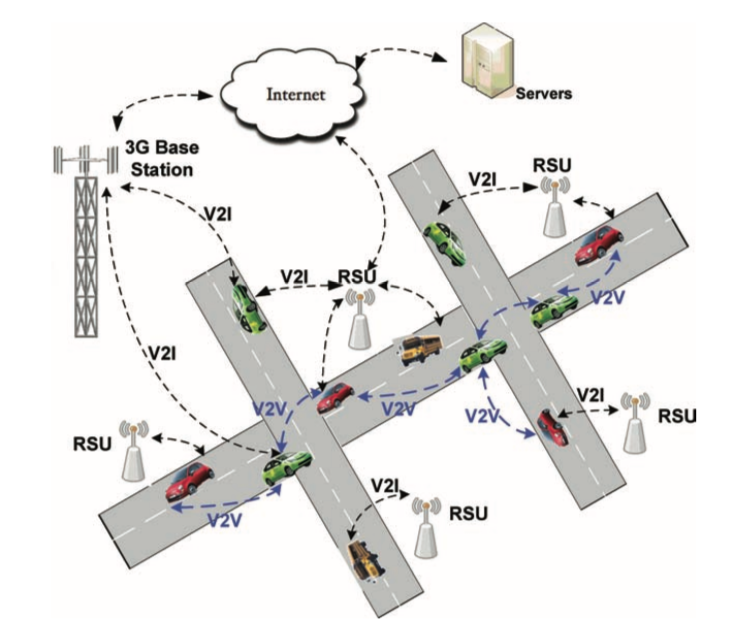
\includegraphics[width=0.95\textwidth]{images/its-modell.png}
  \caption{Modell eine intelligenten Transportsystems\cite{conti2013mobile}.}
  \label{fig:its-modell}
\end{figure}

\section{Taxonomie für VANET-Kommunikationsprotokolle}
\label{sec:taxcommunicationprotocol}
Die Anforderungen an Kommunikationsprotokolle für VANETs variieren enorm und sind stark and unterschiedliche äußerliche Faktoren und Charakteristiken von diesen gebunden.
Im folgenden soll eine Taxonomie basierend auf diesen Faktoren und Charakteristiken für ein solches Protokoll vorgestellt werden.

\subsection{Grundlegende Definitionen}
Bei sogenannter \textit{multihop communication} müssen Nachrichten bzw. Pakete mehrere Zwischenstationen (\textit{hops}) bis zum Empfänger überwinden.
Für die Taxonomie wird diese Kommunikation in drei Kategorien unterteilt:
\begin{itemize}
  \item \textit{routing (one-to-one)}
  \item \textit{geocasting (one-to-all)}
  \item \textit{dissemination (one-to-some)}
\end{itemize}
Die hohe Mobilität der Fahrzeuge im VANET sowie deren variierenden Verbindungen untereinander machen das \textit{routing} zu einer anspruchsvollen Aufgabe.
Mit \textit{routing} lassen sich viele Kommunikationsformen umsetzen, darunter neben \textit{V2V} und \textit{V2I} auch \textit{one-way} und \textit{two-way communication}.
Letzteres erlaubt auch die Kommunikationen zwischen zwei Fahrern oder auch die Reservierung von Parkplätzen.
Um das Problem zu vereinfachen, lassen sich Annahmen über den Empfänger einer Nachricht treffen.
Diese Annahmen können beispielsweise bei einem RSU eine genaue geografische Position sein oder die eines sich bewegenden Fahrzeugs welche natürlich basierend auf Fahrtrichtung und Geschwindigkeit des Fahrzeugs aktualisiert werden muss.
Mit der Nutzung von RSUs als Gateways lässt sich der \textit{routing} Prozess vereinfachen.
Dabei reduziert sich der \textit{routing} Prozess vom Fahrzeug auf das Weiterleiten der Nachricht zum nächsten RSU\@.
Dieser leitet die Nachricht an das RSU weiter, welches sich am nächsten zum Empfänger-Fahrzeug befindet, dieser schlussendlich dann an das Fahrzeug.
Im Weiteren werden RSUs für den \textit{routing} Prozess nicht weiter betrachtet.
Weiterführend lässt sich das \textit{routing} noch weiter unterteilen im Bezug auf die Distanz, die eine Nachricht überwinden muss.
Ist die Distanz beziehungsweise die Position des Empfängers unbekannt spricht man von \textit{FD} (von engl. \textit{finding destination}).
Das Weiterleiten von Nachrichten zwischen zwei Kreuzungen wird unter \textit{small-scale routing (SS)} zusammengefasst.
Geht das \textit{routing} über eine oder mehrere Kreuzungen hinaus, spricht man hingegen von \textit{large-scale routing (LS)}\cite{conti2013mobile}.\\
Beim \textit{broadcasting}, \textit{floading}, \textit{geocasting} oder der \textit{data dissemination} geht es darum eine einzelne Nachricht an mehrere weiteren Knoten in einem Netz zu versenden, wobei die einzelnen Bezeichnungen einen etwas spezifischeren Fall meinen.
Das sogenannte \textit{flooding} konzentriert sich darauf eine einzelne Nachricht immer wieder von allen Empfängern neu zu versenden und damit das Netz zu ``fluten''.
Im Vergleich zum \textit{broadcasting}, bei dem keine räumlichen Grenzen betrachtet werden, sieht das \textit{geocasting} nur die Verbreitung in einem bestimmten Raum vor.
Das \textit{geocasting} kann dabei sowohl von einem Fahrzeug als auch von einem RSU ausgehen und will auf jeden Fall alle Fahrzeuge in einem bestimmten Straßenabschnitt oder Bereich erreichen.
Ein derartiger Bereich kann exemplarisch das Umfeld eines Unfalls sein.
Dabei ist zu beachten, dass der Fokus auf denjenigen Fahrzeugen liegen muss, die sich dem Unfall annähern.
Unter Umständen involviert das \textit{geocasting} auch einen \textit{routing} Prozess zu einem bestimmten Bereich hin, bevor eine Nachricht dann unter allen Fahrzeugen in diesem Bereich verbreitet werden kann\cite{conti2013mobile}.

\subsection{Straßen-Szenario}\label{subsec:strassen-szenario}
Infrastrukturen und Straßenformen wie zum Beispiel Landstraßen oder Autobahnen müssen bezüglich der Kommunikation zwischen einzelnen Automobilen unterschieden werden.
So werden Straßenformen wie die Autobahn welche keine Kreuzungen besitzen als \textit{eindimensional (1D)} bezeichnet.
Ebenso werden Straßen zwischen zwei Kreuzungen als \textit{eindimensional} eingestuft.
Neben der grundlegen eindimensionalen Straßenform existiert ein allgemeineres Szenario mit vielen Kreuzungen an denen Autos abbiegen können und oft die befahrene Straße wechseln.
Solch ein Szenario existiert in vielen Städten und wird als \textit{zweidimensional (2D)} bezeichnet.
Autobahnauffahrten und Kreisverkehre lassen sich keinen der beiden Szenarios eindeutig zuordnen und befinden sich zwischen diesen.
Kommunikationsprotokolle sollten sich im bestmöglichen Fall an den jeweils vorliegenden Straßentyp anpassen.
Protokolle welche für den allgemeineren Fall (2D) entwickelt wurden, können auch für eindimensionale Straßentypen angewendet werden.
Anders herum ist dies nicht ohne weiteres möglich\cite{conti2013mobile}.

\subsection{Benachbarte Fahrzeuge}\label{subsec:benachbarte-fahrzeuge}
Kommunikationsprotokolle lassen sich in hinsichtlich der erforderlichen Kenntnis über benachbarte Fahrzeuge unterteilen.
Hierbei kommen manche Protokolle ohne Kentnisse über andere Fahrzeuge in der Nähe aus (\textit{without neighbor knowledge} oder \textit{NN}).
Im anderen Fall werden periodisch unter allen benachbarten Fahrzeugen Informationen wie Position oder Geschwindigkeit ausgetauscht.
Diese so genannte \textit{neighbor positional knowledge (NP)} wird mittels DSRC (\textit{engl. Dedicated Short-Range Communication}) ausgetauscht.
Bei DSRC handelt es sich um ein MAC-Protokoll (\textit{engl. Medium Access Control}) welches auf einem Frequenzbereich um 5,9 GHz arbeitet\cite{conti2013mobile}.

\subsection{Bestätigung empfangener Nachrichten}
Um sicherzustellen, dass gesendete Nachrichten auch empfangen wurden, können \textit{Acknowledgements} genutzt werden, die den Empfang einer Nachricht bestätigen.
Eine Form um empfangene Nachrichten zu bestätigen sind die sogenannten \textit{beacon acknowledgements} (\textit{BA}).
Hierbei werden stetig in einem festen Abstand \textit{beacons} versendet welche bei erfolgreichem Empfang einer Nachricht diesen bestätigen.
Erhält nun der Sender $S$ ein \textit{beacon} des Empfängers $R$ kann dieser nun eindeutig feststellen welche Nachrichten $R$ bisher empfangen hat.
Diese Methode der Bestätigung funktionieren ebenfalls per direkter Bestätigung, also ohne \textit{beacons}.
Bestätigungen können auch von passiver Form sein (\textit{passive acknowledgement} bzw. \textit{PA}).
Dabei kann der Sender durch den Empfang einer von ihm gesendeten Nachricht, welche somit zwingend weiter verbreitet wurde, Rückschlüsse auf den Empfang dieser ziehen.
Eine weitere Möglichkeit stellt die \textit{reception estimation} (\textit{RE}) dar.
Hierbei basieren Schlüsse vom Sender bezüglich dem Empfang einer Nachricht ausschließlich auf der Distanz zwischen ihm und dem Empfänger der Nachricht.
Manche Protokolle kommen vollkommen ohne \textit{Acknowledgements} aus und werden unter \textit{NA} zusammengefasst\cite{conti2013mobile}.

\subsection{Start des Prozesses zur Weiterleitung von Nachrichten}\label{subsec:forwarder-selection}
Ein Fahrzeug kann sich in zwei verschiedenen Zuständen befinden.
Im \textit{idle} Zustand senden das Fahrzeug keine Nachrichten.
Dies kann entweder eintreteten, falls keine Nachrichten empfangen wurden und somit auch keine weitergeleitet werden können, oder aber durch die Information das alle direkten Nachbarn des Fahrzeugs alle empfangenen Nachrichten bereits erhalten haben.
Befindet sich ein Fahrzeug allerdings im aktiven Zustand (\textit{active}), so können Nachrichten weitergeleitet werden.
Ebenfalls müssen dann diejenigen Nachbarn ausgewählt werden, welche die Nachricht weiter verbreiten sollen.
Für die Entscheidung, wann ein Fahrzeug vom \textit{idle} in den \textit{active} Zustand wechselt, gibt es mehrere Möglichkeiten, die sich allerdings gegenseitig nicht ausschließen und in manchen Protokollen miteinander kombiniert werden.
\subsubsection{\textit{always activate (AA)}}
Fahrzeuge wechseln jedes Mal, wenn sie eine Nachricht erhalten in den aktiven Zustand.
\subsubsection{\textit{immediately activate (IA)}}
Fahrzeuge wechseln nur beim ersten Empfangen einer Nachricht in den aktiven Zustand.
Wird eine Nachricht zum wiederholten Mal empfangen verbleibt das Auto im \textit{idle} Zustand.
\subsubsection{\textit{lack of acknowledgement (LA)}}
Fahrzeuge wechseln in den \textit{active} Zustand, wenn ein \textit{beacon} von einem Nachbarn empfangen wird, in dem die ID einer Nachricht enthalten ist, die der Nachbar nicht erhalten hat.
Dies hat automatisch zur Folge, dass bei dem Eintreffen eines neuen Nachbarn der Zustand des Fahrzeugs immer aktiv wird.
\subsubsection{\textit{neighbor elimination (NE)}}
Ein Fahrzeug $V$ wechselt in den aktiven Zustand, wenn es eine Nachricht von einem Nachbarn $N$ enthält, der nicht alle Nachbarn von $V$ abdeckt.
Ein anderes Fahrzeug $L$ gilt genau dann als von $N$ abgedeckt, falls sich dieses in einem festgelegten Umkreis von $L$ befindet\cite{conti2013mobile}.

\subsection{Übertragung von Nachrichten}
Hat ein Fahrzeug wie in \ref{subsec:forwarder-selection} beschrieben, den aktiven Zustand eingenommen, kann es – muss aber nicht zwingend – Nachrichten weiterverbreiten.
Da die Kommunikation über einem einzigen Kanal läuft, können nicht zwei Knoten gleichzeitig senden, da es sonst zu Kollisionen kommen könnte.
Bedingt dadurch kommt es im Normalfall zu einer Art Wettbewerb zwischen den Fahrzeugen, bei der der Gewinner die Möglichkeit erhält Nachrichten zu versenden.
Die \textit{medium acces control (MAC)}, eine Erweiterung der OSI-Modells, ermöglicht es allerdings Fahrzeugen in kurzen zeitlichen Abständen voneinander zu senden, indem andere Fahrzeuge jeweils auf die Ankunft und damit den Abschluss einer Übertragung warten.
Somit erübrigt sich der Wettbewerb durch die Nutzung der MAC-Schicht, wodurch Protokolle die nur diese Nutzen der Kategorie \textit{NC} bzw. \textit{no competition} angehören.\\
Bei der Nutzung von \textit{DSRC} werden, angelehnt an IEEE 802.11, Zeitslots genutzt, um Kollisionen möglichst zu vermeiden.
Ein Fahrzeug kann senden, wenn sich eine festgelegte Anzahl an freien Zeitslots ergibt.
Dabei kann sich die Wartezeit entweder zufällig ergeben, oder anhand von Prioritäten vergeben werden.
Da die Wartezeit auch zufallsbasiert sein kann, lässt sich keine vollständige Kollisionsfreiheit garantieren und wiederholte Sendungen lassen sich nicht vermeiden.
Broadcasts können durch ihr exponentielles Wachstum (eine Nachricht eines Fahrzeugs wird von mehreren weiterverbreitet) diese Methode hervorragend nutzen.
Für Nachrichten welche jeweils nur von einem einzelnen Fahrzeug zu einem weiteren übertragen werden sollen, existieren bessere Alternativen wie \textit{Ready-to-Send Clear-to-Send} (\textit{RTS-CTS}).
Dabei wird zwischen Sender und Empfänger ein Kanal reserviert, indem der Sender ein RTS-Paket mit der Belegungsdauer für diesen Kanal an den Empfänger sendet, welcher dann zur Bestätigung ein CTS-Paket verschickt.
Erhält der Sender diese Bestätigung, kann er den Kanal sicher kollisionsfrei für den vorgesehenen Zeitraum nutzen.
Bei \textit{RTS-CTS} können ausschließlich Kollisionen beim Senden der RTS- bzw. CTS-Pakete vorkommen, welche in diesem Fall mit zufälliger Wartezeit erneut gesendet werden können.
\textit{Ready-to-Send Clear-to-Send} ist ein Protokoll welches der Kategorie \textit{time delay} (\textit{TD}) angehört.\\
Mit \textit{black burst} (\textit{BB}) existiert eine weitere Option bei der Knoten die eine Nachricht senden wollen ein Rauschsignal ausgeben und erst dann die Nachricht senden, wenn sie kein Rauschsignal von anderen Knoten empfangen\cite{conti2013mobile}.

\subsection{Konnektivität}
Der temporäre Verlust der Verbindung zwischen Fahrzeugen oder RSUs stellt für manche Kommunikationsprotokolle ein Problem dar, da diese auf der Annahme einer ständigen Verbindung aufbauen.
Sollten Schwierigkeiten bei der Verbindung auftauchen, können Durchsatz und Zuverlässigkeit eines solchen Protokolls stark schwanken.
Für ein Szenario in dem eine ständige Verbindung vorausgesetzt wird, kommt der Begriff \textit{always connected} (\textit{AC}) zum Einsatz.
Andere Protokolle betrachten ein anderes Szenario, \textit{intermittent connectivity} (\textit{IC}), in dem es zu temporären Aussetzern bei der Verbindung kommen kann, wodurch diese bei Konnektivitätsproblemen weniger Einbußen bei der Performance haben.
Diese Resistenz gegen Verbindungsausfälle kann unter anderem mit dem Zwischenspeichern von Nachrichten erreicht werden\cite{conti2013mobile}.


\subsection{Dringlichkeit von Nachrichten}
Die \textit{Dringlichkeit} beim Versenden einer Nachricht kann voneinander abweichen.
Eine Nachricht, welche vor einen Unfall in unmittelbarer Nähe warnt, erfordert eine möglichst kurze Zeit für die Übertragung.
Das derartige Versenden von Nachrichten wird als \textit{zeitkritisch} (\textit{TC} von engl. \textit{time critical}) bezeichnet.
Es ist zu beachten, dass die Benachrichtigung für Fahrzeuge in der Nähe nur zeitkritisch ist, falls diese sich in Richtung des Unfalls bewegen.
Im Gegensatz zu den zeitkritischen Nachrichten stehen die sogenannten \textit{zuverlässigkeits-orientierten} (\textit{RO} von engl. \textit{reliability-oriented}) Nachrichten.
Hierbei liegt der Fokus darauf, dass alle Fahrzeuge, welche die Nachricht bekommen sollen, diese auch erhalten.
Ein Beispiel hierfür ist das Erhalten einer Werbung für eine Tankstelle in einem bestimmten Umkreis von dieser\cite{conti2013mobile}.

\subsection{Nachrichten}
Für Weiterleitung von Nachrichten in einem VANET enthalten diese neben dem eigentlichen Informationsgehalt zusätzliche Informationen.
Algorithmen zur Weiterleitung von jenen Nachrichten treffen unterschiedliche Annahmen welche solcher Informationen enthalten sind.
Hierbei wird hauptsächlich zwischen zwei Kategorien von Nachrichten unterschieden.
Eine sogenannte \textit{vollständige Nachricht} (\textit{FM} von engl. \textit{full message}) kann Informationen wie Versender, dessen Geschwindigkeit und Position, so wie den genauen Empfänger enthalten.
Im Gegensatz dazu stehen Nachrichten, bei denen die Knoten, welche die Nachricht weiterleiten sollen, in der Nachricht enthalten sind.
Diese Nachrichten werden unter \textit{forwarder attached} (\textit{FA}) zusammengefasst.
Algorithmen die auf \textit{FA} basieren gelten als \textit{Sender orientiert}, da jeweils der Sender der Nachricht darüber entscheidet, welcher Empfänger-Knoten die Nachricht weiterleitet.
Aufgrund der fehlenden Kenntnis des Senders über die Nachbarknoten der Empfänger, ist der Sender nicht dazu in der Lage, die bestmöglichen Entscheidungen darüber treffen welcher Empfänger die Nachricht weiterleiten soll.
Umgekehrt gelten die auf \textit{FM} basierenden Algorithmen als \textit{Empfänger orientiert} und sind generell deutlich zuverlässiger\cite{conti2013mobile}.



\section{Kommunikationsprotokolle für VANETs}
\label{sec:protocols}
Im Folgenden soll näher auf einzelne VANET-Kommunikationsprotokolle eingegangen werden und diese im Hinblick auf die vorgestellte Taxonomie eingeordnet werden.
Hierbei wird die Funktionsweise für ein Protokoll im Detail beschrieben sowie der mögliche Anwendungsbereich des Protokolls.
Zudem sollen mögliche Schwachstellen der einzelnen Protokolle aufgezeigt werden und ein beispielhafter Kommunikationsablauf beschrieben werden.
Abschließend findet sich eine tabellarische Übersicht der Protokolle im Bezug auf die Taxonomie\cite{conti2013mobile}.

\subsection{Zuverlässiges und effizientes Broadcasting in VANETs (ackPBSM)}
Bei \textit{ackPBSM} (von engl. \textit{parameterless reliable broadcasting strategy with acknowledgement}) handel es sich um eine zuverlässige Strategie für Broadcasts welche keine Parameter nutzt und \textit{Acknowledgements} zur bestätigung von Nachrichten nutzt.
Ziel des Protokolls sind eine hohe Zuverlässigkeit beim Versenden von Nachrichten sowie die Reduzierung der benötigten Nachrichten zum weiterverbreiten der Nachricht.
Dabei ist \textit{ackPBSM} unabhängig vom Straßen-Szenario aus \ref{subsec:strassen-szenario} und funktioniert sowohl für \textit{eindimensionale} als auch für \textit{zweidimensionale} Szenarios.
Das Protokoll nutzt \textit{beacon acknowledgements} (\textit{BA}) um Informationen über andere Fahrzeuge zu gewinnen, welche die Postion des Senders sowie Bestätigungen von erhaltenen Nachrichten enthalten.
Um insgesamt möglichst wenige Nachrichten für einen Broadcast zu benötigen wird ein \textit{minimaler Spannbaum} erzeugt.
Dies geschieht, indem jedes Fahrzeug periodisch eine Art Start-Nachricht versendet (oder ein \textit{beacon}) woraus daraufhin ohne weiteren Overhead eine \textit{untereinander verbundene domierende Menge} (\textit{CDS} von engl. \textit{connected dominating set}) erzeugt werden kann.
Eine \textit{untereinander verbundene domierende Menge} enthält eine minimale Anzahl an Knoten, sodass jeder Knoten im Netz entweder selbst Teil dieser ist oder Nachbar eines Knoten ist, welche in der \textit{untereinander verbundenen domierenden Menge} enthalten ist.
Zudem müssen alle Knoten, die Teil des \textit{CDS} sind, untereinander ebenfalls verbunden sein.
Dies stellt unter anderem sicher, dass nach einer Nachricht von einem beliebigen Knoten $V$ sich diese im ganzen Netz verbreitet wenn nur Knoten des \textit{CDS} die Nachricht an alle Nachbarn verbreiten.
Die Nachricht erreicht sicher das \textit{CDS}, da $V$ entweder selbst Teil des \textit{CDS} sein muss oder mindesten einen Nachbarn besitzen muss der diese Eigenschaft erfüllt.
Durch die Nutzung einer \textit{untereinander verbundenen domierenden Menge} lassen sich Kollisonen von Nachrichten reduzieren, da insgesamt weniger Nachricht versendet werden müssen für einen Broadcast.
Dies ist besonders nützlich in dichten Netzwerken die sich besonders in Staus oder beim Warten vor einer Ampel bilden.
Es ist zu beachten, dass alle Knoten im Netz zusammen auch ein \textit{CDS} ergeben und die \textit{untereinander verbundene domierende Menge} zur optimalen Nutzung möglichst minimal sein sollte\cite{conti2013mobile}.\\
Bei der Nutzung von \textit{ackPBSM} besitzt jedes Fahrzeug $C$ zwei Listen:
\begin{itemize}
  \item \textit{R} enthält diejenigen Nachbarn, von denen $C$ annimmt, dass sie die Nachricht erhalten haben.
  \item \textit{N} enthält alle anderen direkten Nachbarn von $C$.
\end{itemize}
Fall $C$ eine Nachricht zum wiederholten mal empfängt, werden alle Fahrzeuge welche aufgrund ihrer aktuellen Position die Nachricht ebenfalls erhalten haben sollten, zu \textit{R} hinzugefügt.
Die Zeit in der entschieden wird, ob eine Nachricht von einem Knoten im \textit{CDS} weiterverbreitet wird, ist antiproportional zur Anzahl von Knoten in \textit{N}.
Das bedeutet je mehr direkte Nachbarn eines Knotens $C$ eine Nachricht vermutlich nicht erhalten haben, desto kürzer ist die Wartezeit bis zum weiterbreiten der Nachricht von $C$.
Knoten welche sich nicht im \textit{CDS} befinden, besitzen allgemein eine längere Wartezeit.
Bei \textit{ackPBSM} wird \textit{neighbor elimination (NE)} genutzt, da Fahrzeuge eine Nachricht nur dann weiterverbreitet wird, wenn sich mindestens ein Fahrezug in der Liste \textit{N} befindet.
Befindet sich nun mindesten ein Fahrzeug in \textit{N} wird die Nachricht versendet und alle Nachbarn werden in \textit{R} verschoben.
Ein Fahrzeug $D$ kann von \textit{R} zurück nach \textit{N} verschoben werden, falls der Sender keine Bestätigung von $D$ über den Empfang der Nachricht erhält.
\textit{ackPBSM} überwindet auch temporäre Verluste der Verbindung eines Fahrzeugs durch das Zwischenspeichern von Nachrichten und betrachtet somit das Szenario \textit{intermittent connectivity} (\textit{IC})\cite{conti2013mobile}.\\
Bei \textit{ackPBSM} tauscht jedes Fahrzeug Informationen mit seinen direkten Nachbarn aus und lässt sich nach \ref{subsec:benachbarte-fahrzeuge} in die Kategorie \textit{NP} einordnen.
Um einen detaillierteren Einblick in das Protokoll zu bieten, wird in \ref{fig:ackpbsm-example} ein beispielhafter Ablauf eines Broadcasts mit \textit{ackPBSM} dargestellt.

\begin{figure}[h]
  \centering
  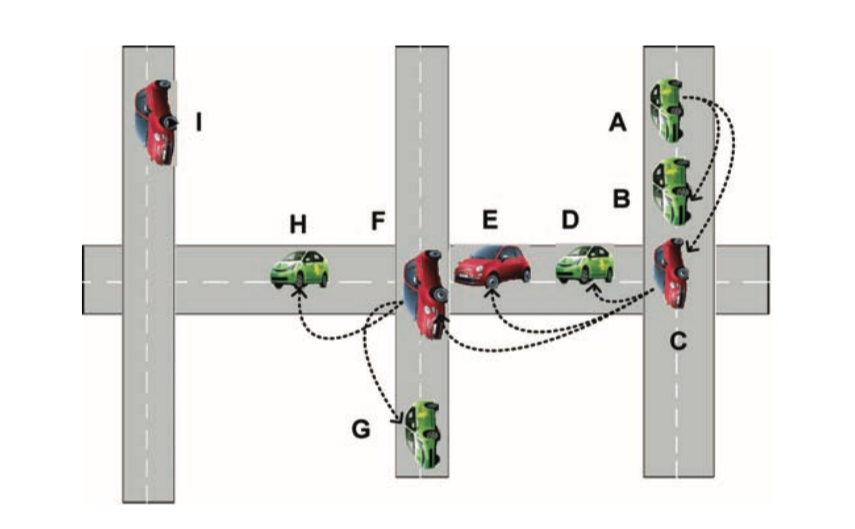
\includegraphics[width=0.95\textwidth]{images/ackpbsm-example.png}
  \caption{Beispiel eines Broadcasts mit \textit{ackPBSM}\cite{conti2013mobile}.}
  \label{fig:ackpbsm-example}
\end{figure}

Bevor Fahrzeug $A$ seinen Broadcast startet, wird das \textit{CDS} gebildet.
Dabei gehören im Beispiel die Fahrzeuge $C$, $E$, $F$ und $I$ (markiert in rot) zum \textit{CDS}.
$A$ versendet die Nachricht an alle Fahrzeuge in seiner unmittelbaren Umgebung ($B$ und $C$), wobei $B$ die Nachricht nicht direkt weiterverbreitet und im aktiven Zustand verweilt, da $B$ davon ausgeht, dass $C$, aufgrund seiner Position, die Nachricht aufgrund ebenfalls erhalten hat.
$C$ hingegen besitzt einen Nachbarn ($D$) der die Nachricht vermutlich nicht erhalten hat (\textit{NE}) und verbreitet die Nachricht somit weiter.
Da $B$ nun die Nachricht erneut erhält, wird der aktive Zustand verlassen und die Weiterverbreitung gestoppt.
Außerdem erhalten neben $B$ auch $D$, $E$ und $F$ die Nachricht.
Da $E$ und $F$ Teil des \textit{CDS} sind, kommen diese für die Weiterverbreitung zuerst in Frage, wobei $F$ zuerst sendet da die Wartezeit antiproportional zu der Anzahl an Nachbarn ist, welche die Nachricht noch nicht erhalten haben ($H$ und $G$).
Wenn $F$ nun die Nachricht weiterleitet, verlassen $E$ und $D$ den aktiven Zustand da sie die Nachricht zum wiederholten Male (nun von $F$) empfangen.
Da $I$ nicht in Reichweite eines Fahrzeugs ist, kann es die Nachricht erst erhalten wenn zum Beispiel $H$ weiter fährt und sich somit $I$ annähert.
Durch einen \textit{beacon} von $I$ erhält $H$ dann die Information, dass $I$ die Nachricht noch nicht erhalten (\textit{LA}) hat und kann diese, da sie zwischengespeichert wurde, (\textit{IC}) erneut senden.
Durch die Bestätigungen über den Empfang der Nachricht ist \textit{ackPBSM} sehr zuverlässig, da im Falle eines Nicht-Erhaltens die Nachricht einfach erneut gesendet werden kann.
Zudem werden auch im Falle von Überholmannövern, wodurch neue Nachbarn aufkommen, welche die Nachricht allerdings schon kennen, keine zusätzlichen versendet, da mit den \textit{beacon} der Empfang bestätigt wird und somit direkt Informationen über alle erhaltenen Nachrichten von neuen Nachbarn erhalten werden.\\
Ein Nachteile von \textit{ackPBSM} ergibt sich aus dem Overhead der durch die stets gesendeten Bestätigungen, die weitere Daten mit sich führen, entsteht.
Für eine zeitkritische Nutzung des Protokolls müsste die Funktion für die zeitliche Verzögerung beim Weiterverbreiten einer Nachricht genauer spezifiert werden\cite{conti2013mobile}.

%\subsection{Persistance-Based Protocols}
%\subsection{Multihop Vehicular Broadcast (MHVB)}
%\subsection{Emergency Message Dissemination with ACK-Overhearing Based Retransmission (EMDOR)}
%\subsection{Distributed Fair Power Adjustment Protocol (D-FPAV)}
%\subsection{Receiver Consensus (ReC)}
%\subsection{DPP und OPERA}
%\subsection{Binary-Partition-Assisted Broadcast (BPAB)}
%\subsection{Track Detection und Distance Defer Transmission Protocols (TRADE und DDT)}
%\subsection{Connection-Based Restricted Forwarding (CBRF)}
%\subsection{Distributed Vehicular Broadcast (DV-CAST)}
%\subsection{Vehicle Density-Based Emergency Broadcasting (VDEB)}
%\subsection{Topology-Assisted Geo-Opportunistic Routing (TO-GO)}
%\subsection{Distance-Aware Epidemic Routing (DAER)}
%\subsection{Connectivity-Aware Routing (CAR)}
%\subsection{Delay-Bounded Routing in VANETs (D-Greedy)}
%\subsection{Vehicle-Assisted Data Delivery in VANETs (VADD)}
%\subsection{Trajectory-Based Data Forwarding for Light-Traffic in VANETs (TBD)}
%\subsection{Static-Node-Assisted Adaptive Routing Protocol in VANETs (SADV)}
%\subsection{Location- and Delay-Aware Cross-Layer Communication (LD-CROP)}
%\subsection{Geopgraphical Opportunistic Routing (GeoOpps)}
%\subsection{Road-Based Vehicular Traffic Routing (RBVT)}
%\subsection{Improved Greedy Traffic-Aware Routing Protocol (GyTAR)}
%\subsection{Acces-Overlay Routing by Two-Phase Routing Protocol (TOPO)}

\section{Zusammenfassung und Fazit}
\label{sec:conclusion}
VANETs können das Verkehrsgeschehen überaus positiv auf unterschiedlichste Arten beeinflussen.
Die Kommunikation zwischen einzelnen Fahrzeugen und von Fahrzeugen zu anderer Infrakstruktur ist hierzu unerlässlich.
Um bestehende Kommunikationprotokolle einordnen zu können und eine Orientierung für die Entwicklung von neuen Protokollen bieten zu können, wurde eine Taxonomie für diese vorgestellt.
Zudem lassen sich mit der Taxonomie die Grenzen von einzelnen Protokollen leicht erkennen.
So lassen sich wie in \ref{subsec:strassen-szenario} beschrieben, Protokolle für ein \textit{eindimensionales} Szenario nicht auf alle realen Applikationen ohne weiteres anwenden.
Daraufhin wurden verschiedene Protokolle vorgestellt und im Hinblick auf die Taxonomie eingeordnet.
Eine Übersicht mit den vorgestellten sowie mehreren weiteren Protokollen findet sich in \ref{table:1} in kompakter Form\cite{conti2013mobile}.

\begin{table}[]
    \begin{tabular}{llllllllll}
     \toprule
    Protokoll                     & Problem Statement     & Transmission Dimension    & Neighbor Knowledge     & Acknowledgement     & Starting Forwarder Selection    & Compete to Retransmit & Connectivity & Urgency & Message Content \\
     \midrule
     Probabilistic, naive flooding & G        & 2D & NN    & NA & AA     & NC       & IC    & RO & FM \\
    Middle                        & G        & 1D & NN    & NA & IA     & TD-D     & AC    & RO & FA \\
    ackPBSM                       & G        & 2D & NP    & BA & LA, NE & TD-D     & IC    & RO & FM \\
    Persistence                   & G        & 1D & NN    & PA & IA     & TD-D     & AC    & RO & FM \\
    MHVB                          & G        & 1D & NN    & PA & NE     & TD-D     & AC    & TC & FM \\
    EMDOR                         & G        & 1D & NN    & BA & IA, LA & TD-D     & AC    & TC & FA \\
    EMDV                          & G        & 2D & NP    & RE & IA     & TD-D     & AC    & TC & FA \\
    ReC                           & G        & 2D & NP    & BA & IA     & TD-D     & IC    & TC & FM \\
    OPERA                         & R-SS     & 1D & NP    & BA & LA, NE & X        & IC    & TC & FM \\
    BPAB                          & R-SS     & 1D & NN    & PA & NE     & BB, TD-R & AC/IC & TC & FA \\
    TRADE/DDT                     & R-SS     & 1D & NP/NN & NA & IA     & TD-D     & AC    & RO & FA \\
    CBRF                          & R-SS     & 1D & NN    & BA & IA     & TD-R     & AC    & TC & FA \\
    DDP                           & R-SS     & 1D & NP    & BA & IA     & TD-D     & IC    & TC & FM \\
    DV-CAST                       & R-SS     & 1D & NP    & PA & IA     & TD-D     & AC    & RO & FM \\
    VDEB                          & R-SS     & 1D & NP    & BA & I      & TD-D     & AC    & TC & FA \\
    TOGO                          & R-LS     & 1D & NP    & BA & IA     & TD-D     & IC    & RO & FM \\
    DAER                          & R-FD, LS & 2D & NP    & BA & IA     & TD-D     & AC    & RO & FM \\
    CAR                           & R-LS     & 2D & NP    & BA & IA     & TD-R     & IC    & RO & FM \\
    D-greedy                      & R-LS     & 2D & NP    & BA & IA     & TD-D     & IC    & TC & FM \\
    VADD                          & R-LS     & 2D & NP    & BA & IA     & TD-D     & IC    & TC & FM \\
    TBD                           & R-LS     & 2D & NP    & BA & IA     & TD-R     & IC    & TC & FM \\
    SADV                          & R-LS     & 2D & NP    & BA & IA     & TD-D     & IC    & TC & FM \\
    LD-CROP                       & R-LS     & 2D & NP    & BA & IA     & TD-R     & IC    & RO & FM \\
    GeOpps                        & R-LS     & 2D & NP    & BA & IA     & TD-D     & IC    & TC & FA \\
    RBVT                          & R-FD, LS & 2D & NP    & BA & IA     & TD-D     & AC    & RO & FA \\
    GyTAR                         & R-LS     & 2D & NP    & BA & IA     & TD-D     & IC    & RO & FA \\
    TOPO                          & R-LS     & 2D & NP    & BA & IA     & TD-R     & IC    & RO & FA \\
     \bottomrule
    \end{tabular}
  \caption{Übersicht über verschiede Kommunikationsprotokolle für VANETs\cite{conti2013mobile}}
  \label{table:1}
\end{table}

\subsubsection*{Acknowledgments}
\ldots

In the bibliography, use \texttt{\textbackslash textsuperscript} for \qq{st}, \qq{nd}, \ldots:
E.g., \qq{The 2\textsuperscript{nd} conference on examples}.
When you use \href{https://www.jabref.org}{JabRef}, you can use the clean up command to achieve that.
See \url{https://help.jabref.org/en/CleanupEntries} for an overview of the cleanup functionality.

\renewcommand{\bibsection}{\section*{References}} % requried for natbib to have "References" printed and as section*, not chapter*
% Use natbib compatbile splncsnat style.
% It does provide all features of splncs03, but is developed in a clean way.
% Source: http://phaseportrait.blogspot.de/2011/02/natbib-compatible-bibtex-style-bst-file.html
\bibliographystyle{splncsnat}
\begingroup
  \ifluatex
    %try to activate if bibliography looks ugly
    %\sloppy
  \else
    \microtypecontext{expansion=sloppy}
  \fi
  \small % ensure correct font size for the bibliography
  \bibliography{paper}
\endgroup

% Enfore empty line after bibliography
\ \\
%
Alle Links wurden zuletzt am 20. Januar 2021 abgerufen.
\end{document}
